\documentclass[11pt]{article}
\usepackage[a4paper,top=1.5cm,bottom=3.0cm,left=1.9cm,right=1.9cm,footskip=2.0cm]{geometry}
\usepackage{graphicx}
\usepackage[table]{xcolor}
\usepackage{ragged2e}
\usepackage{fancyhdr}
\usepackage{fontspec}
\setmainfont{Noto Sans Kannada}
\setsansfont{Noto Sans Kannada}
\newfontfamily\latinfont{Carlito}
\renewcommand{\familydefault}{\sfdefault}
\definecolor{titleblue}{HTML}{0F2F4A}
\definecolor{textblack}{HTML}{1A1A1A}
\definecolor{rule}{HTML}{C9C4C0}
\definecolor{muted}{HTML}{6B635E}
\setlength{\parindent}{0pt}\setlength{\parskip}{0.5em}

\setlength{\headheight}{0pt}\setlength{\headsep}{0pt}
\pagestyle{fancy}
\fancyhf{}
\renewcommand{\headrulewidth}{0pt}
\renewcommand{\footrulewidth}{0pt}
\fancyfoot[C]{%
  \begin{minipage}{\textwidth}
    {\color{rule}\hrule height 0.7pt}\vspace{4pt}
    \noindent
    \begin{minipage}[c]{0.66\textwidth}{\scriptsize\color{muted}{\latinfont Developed by the Water and Climate Lab, IIT Gandhinagar, using hydro-meteorological data from IMD and partner agencies}.}\end{minipage}\hfill
    \begin{minipage}[c]{0.32\textwidth}\raggedleft
      
\includegraphics[height=0.62cm]{wcl.png}\hspace{6pt}%
      
\includegraphics[height=0.62cm]{iitgn.png}\hspace{6pt}%
      
\includegraphics[height=0.62cm]{imd.png}
    \end{minipage}\\[3pt]
    {\scriptsize\color{muted}© {\latinfont 2026 Water and Climate Lab} · {\latinfont Indian Institute of Technology Gandhinagar} · {\latinfont For research and demonstration purposes}.}
  \end{minipage}%
}

\begin{document}

\noindent
\begin{minipage}[c]{0.16\textwidth}
\includegraphics[width=\linewidth]{wcl.png}\end{minipage}\hfill
\begin{minipage}[c]{0.80\textwidth}\raggedleft
  {\fontsize{19}{22}\selectfont\bfseries\color{titleblue}{\latinfont National Drought Summary}}\\[2pt]
  {\normalsize\color{muted}{\latinfont Week ending May 20, 2026}}
\end{minipage}
\vspace{6pt}{\color{rule}\hrule height 1pt}\vspace{10pt}
\begin{center}
  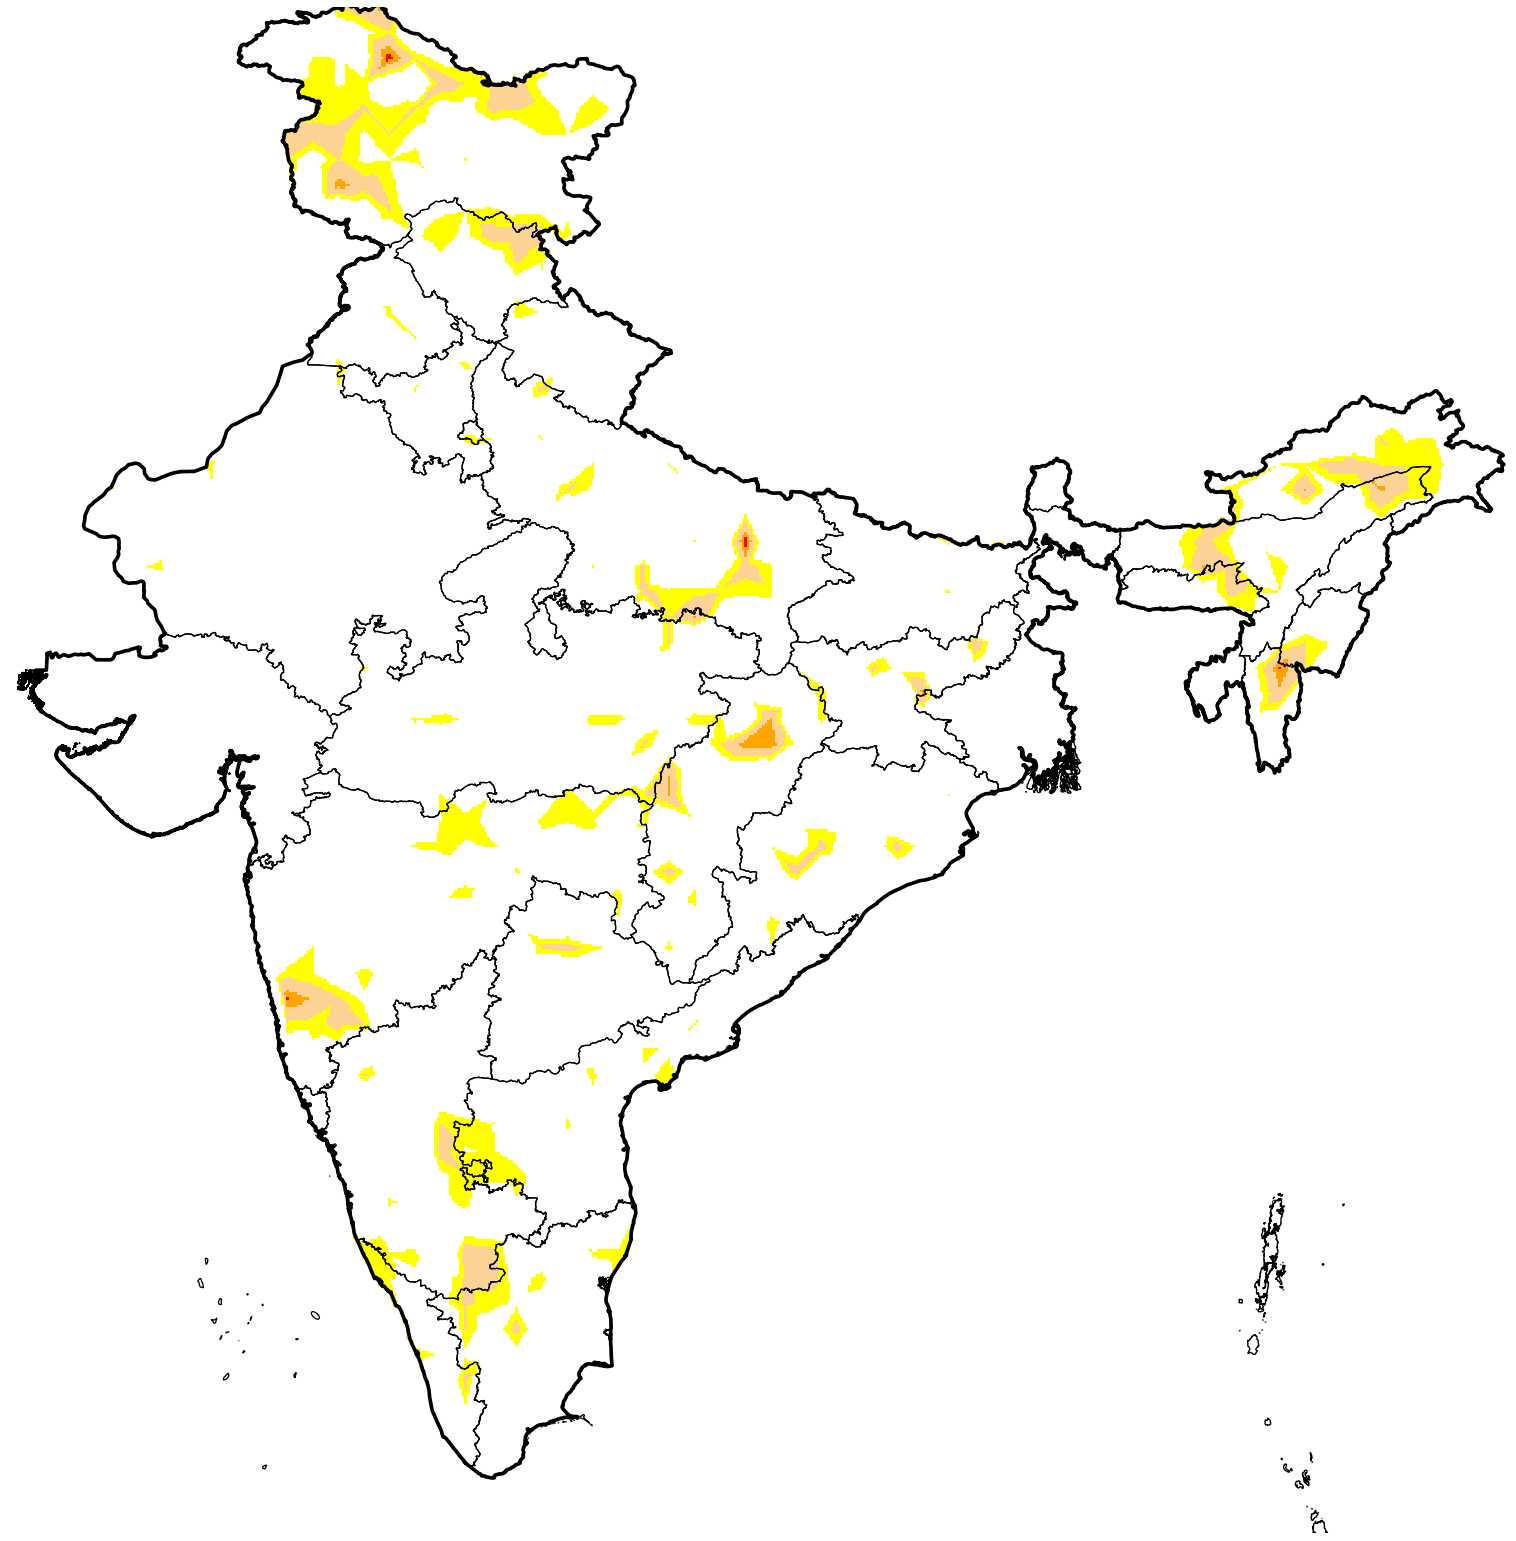
\includegraphics[width=0.60\textwidth]{cdi_map.png}\\[3pt]
  {\small\color{muted}{\latinfont Combined Drought Index (CDI) for the week ending May 20, 2026}.}
\end{center}
\vspace{2pt}
{\large\bfseries\color{titleblue}{\latinfont Summary}}\\[3pt]
{\justifying\normalsize\color{textblack}ಈ ವಾರದ ರಾಷ್ಟ್ರೀಯ ಬರ ಪರಿಸ್ಥಿತಿಯು ಭಾರತದ ಹೆಚ್ಚಿನ ಭಾಗವು ಸಾಮಾನ್ಯ ವಿಭಾಗದಲ್ಲಿ ಉಳಿದಿದೆ ಎಂದು ತೋರಿಸುತ್ತದೆ,যেখানে {\latinfont 84.7}\% ಪ್ರದೇಶವನ್ನು ಸಾಮಾನ್ಯ ಎಂದು ವರ್ಗೀಕರಿಸಲಾಗಿದೆ. ಈ ವಾರ ಬರ ಪರಿಸ್ಥಿತಿಗಳನ್ನು ಅನುಭವಿಸುತ್ತಿರುವ ಒಟ್ಟು ಪ್ರದೇಶ, ನಿರ್ದಿಷ್ಟವಾಗಿ ಡಿ{\latinfont 0} ಮತ್ತು ಅದಕ್ಕಿಂತ ಹೆಚ್ಚು, {\latinfont 15.3}\% ಆಗಿತ್ತು. ಈ ಅಂಕಿಅಂಶವು ಹಿಂದಿನ ಅವಧಿಗಳಿಗೆ ಹೋಲಿಸಿದರೆ ಬರ ಪ್ರದೇಶದಲ್ಲಿ ಸಂಕೋಚನವನ್ನು ಪ್ರತಿಬಿಂಬಿಸುತ್ತದೆ, ಏಕೆಂದರೆ ಒಟ್ಟು ಬರ ಪ್ರದೇಶ ವಾರದಿಂದ ವಾರಕ್ಕೆ {\latinfont 0.9} ಶೇಕಡಾ ಅಂಕಗಳನ್ನು ಕಡಿಮೆಗೊಂಡು, ಕಳೆದ ವಾರದ {\latinfont 16.2}\% ರಿಂದ ಪ್ರಸ್ತುತ {\latinfont 15.3}\% ಕ್ಕೆ ಇಳಿದಿದೆ. ಬರದಿಂದ ಹೆಚ್ಚು ಬಾಧಿತವಾಗಿರುವ ಪ್ರದೇಶಗಳು ದೆಹಲಿ ರಾಷ್ಟ್ರಕ{\latinfont uml} ಪ್ರದೇಶವಾಗಿದ್ದು, ಅದರ {\latinfont 52.2}\% ಪ್ರದೇಶವು ಬರದಲ್ಲಿ ಇದೆ, ನಂತರ ಮಣಿಪುರದಲ್ಲಿ {\latinfont 42.3}\%, ಮಿಜೋರಾಂನಲ್ಲಿ {\latinfont 40.8}\%, ಅರುಣಾಚಲ ಪ್ರದೇಶದಲ್ಲಿ {\latinfont 40.3}\%, ಜಮ್ಮು ಮತ್ತು ಕಾಶ್ಮೀರದಲ್ಲಿ {\latinfont 38.9}\%, ಮತ್ತು ಮೇಘಾಲಯದಲ್ಲಿ {\latinfont 34.1}\% ಇದೆ. ಇದಕ್ಕೆ ವ್ಯತಿರಿಕ್ತವಾಗಿ, ಪಶ್ಚಿಮ ಬಂಗಾಳವು ತನ್ನ ಪ್ರದೇಶದ {\latinfont 0.0}\% ಬರ ಎಂದು ವರದಿ ಮಾಡಿದೆ, ಆದರೆ ರಾಜಸ್ಥಾನವು ತನ್ನ ಪ್ರದೇಶದ {\latinfont 1.0}\% ಬರದಿಂದ ಅತ್ಯಂತ ಕಡಿಮೆ ಬಾಧಿತ ರಾಜ್ಯವಾಗಿದೆ.\par}
\vspace{8pt}
{\large\bfseries\color{titleblue}{\latinfont Regional Outlook}}\\[2pt]
{\normalsize\color{titleblue}\textbf{{\latinfont North}}}\enspace {\normalsize\color{textblack}{\latinfont Moderate, scattered drought. About 28}\% {\latinfont of the area is in drought (D0}–{\latinfont D4)}.} \par\smallskip {\normalsize\color{titleblue}\textbf{{\latinfont Northwest}}}\enspace {\normalsize\color{textblack}{\latinfont Largely normal conditions. About 4}\% {\latinfont of the area is in drought (D0}–{\latinfont D4)}.} \par\smallskip {\normalsize\color{titleblue}\textbf{{\latinfont Northeast}}}\enspace {\normalsize\color{textblack}{\latinfont Moderate, scattered drought. About 27}\% {\latinfont of the area is in drought (D0}–{\latinfont D4). Pockets of severe-or-worse conditions are present}.} \par\smallskip {\normalsize\color{titleblue}\textbf{{\latinfont East}}}\enspace {\normalsize\color{textblack}{\latinfont Mostly normal, with localised dryness. About 7}\% {\latinfont of the area is in drought (D0}–{\latinfont D4)}.} \par\smallskip {\normalsize\color{titleblue}\textbf{{\latinfont Central}}}\enspace {\normalsize\color{textblack}{\latinfont Mostly normal, with localised dryness. About 15}\% {\latinfont of the area is in drought (D0}–{\latinfont D4). Pockets of severe-or-worse conditions are present}.} \par\smallskip {\normalsize\color{titleblue}\textbf{{\latinfont West}}}\enspace {\normalsize\color{textblack}{\latinfont Moderate, scattered drought. About 22}\% {\latinfont of the area is in drought (D0}–{\latinfont D4)}.} \par\smallskip {\normalsize\color{titleblue}\textbf{{\latinfont South}}}\enspace {\normalsize\color{textblack}{\latinfont Mostly normal, with localised dryness. About 16}\% {\latinfont of the area is in drought (D0}–{\latinfont D4)}.}
\end{document}
